\documentclass[11pt]{article}
\usepackage[margin=1in]{geometry}
\usepackage{amsmath,amssymb}
\usepackage{graphicx}
\usepackage{booktabs}
\usepackage{xcolor}
\usepackage[hidelinks]{hyperref}
\usepackage{natbib}
\usepackage{caption}
\captionsetup{font=small}
\graphicspath{{figures/}}

\newcommand{\pe}{\textsc{PromptEval}}

\title{\bf Reliable in the Center, Unreliable at the Edges:\\
Auditing the Tail Fragility of Multi-Prompt LLM Evaluation}
\author{}
\date{}

\begin{document}
\maketitle

\begin{abstract}
Because large language model (LLM) accuracy varies sharply with the exact wording of a
prompt, a growing line of work replaces single-prompt scores with an estimate of the
\emph{distribution} of accuracy across many prompt templates. \pe{}
\citep{polo2024prompteval}, a NeurIPS 2024 method built on a regularized Rasch model, is a
prominent and widely reused instance: it estimates performance quantiles across 100
templates at ``the budget of two single-prompt evaluations.'' We first reproduce \pe{}
exactly---our re-implementation matches the authors' released MMLU quantile-error array to
four decimal places. We then stress-test the claim that matters most in practice: how well
does it estimate the \emph{tails} of the prompt-accuracy distribution (worst- and best-case
prompts), which are precisely why one runs a multi-prompt evaluation? We find a large,
systematic, and previously unreported \textbf{center--tail reliability gap}. At the advertised
budget, median-quantile error is a negligible $0.05$, but the $5$th/$95$th percentile error is
$4.2\times$ larger ($95\%$ CI $[4.05,4.45]$; Wilcoxon $p\!\approx\!10^{-141}$ over $855$
subject$\times$model cells), and---counterintuitively for a regularized estimator---the
error is \emph{directional}: the worst prompt is estimated far too low and the best prompt too
high, so the estimated prompt-sensitivity spread is inflated (median $8.4\times$ the truth).
The gap does not close with budget; the tail/center error ratio actually \emph{grows} from
$4.2\times$ to $10\times$ as the budget increases, because the center converges faster. We
trace the effect to finite-sample over-dispersion and introduce a \textbf{self-contained
deconvolution correction} that estimates the noise-induced spread inflation from the budgeted
data alone and shrinks the estimated distribution accordingly, cutting tail error by
$\sim\!64\%$ without additional labels. Our results are a cautionary, actionable refinement of
multi-prompt evaluation: trust its center, correct or distrust its tails. All code and
re-analysis run on a laptop and reproduce from the authors' public data.
\end{abstract}

\section{Introduction}
LLM benchmark scores are notoriously sensitive to superficial prompt choices: reformatting a
question or reordering options can shift accuracy by tens of points
\citep{sclar2024quantifying,mizrahi2024state}. A single fixed template therefore reports a
point on a wide, unknown distribution. \pe{} \citep{polo2024prompteval} addresses this by
estimating the \emph{full distribution} of accuracy across a large template set under a small
evaluation budget, using an extended Rasch (item-response) model that borrows statistical
strength across templates and items. Its headline result is that performance \emph{quantiles}
across $100$ MMLU templates can be recovered ``with a budget equivalent to two single-prompt
evaluations.'' The method is influential and is already reused as a data source by downstream
work \citep{rankintervals2026}.

The practical appeal of a full distribution is not the mean---a single prompt already
estimates that---but the \emph{tails}: What is my worst-case prompt? How prompt-robust is my
model? Which template is best? These are questions about the extreme quantiles. We therefore
ask a simple stress-test question: \emph{is \pe{} as reliable at the tails as its headline
suggests?}

We make four contributions.
\begin{enumerate}\itemsep2pt
\item \textbf{Exact reproduction.} Our independent re-implementation reproduces the authors'
released MMLU quantile-error results to four decimals (max cell difference $0.0000$), giving a
trustworthy basis for further analysis (\S\ref{sec:repro}).
\item \textbf{A center--tail reliability gap.} At the advertised budget, extreme-quantile error
is $4.2\times$ the median error, overwhelmingly significant, and the ratio \emph{grows} with
budget (\S\ref{sec:gap}). The single averaged error metric reported in prior work hides this.
\item \textbf{A directional mechanism.} The tail error is not symmetric noise but systematic
\emph{over-dispersion}: the estimated distribution is wider than the truth, so worst-case
performance is overstated and prompt-robustness understated (\S\ref{sec:mech}). We attribute
it to finite-sample inflation and show the spread ratio decays monotonically toward $1$ with
budget.
\item \textbf{A self-contained correction.} A parametric-bootstrap deconvolution estimates the
inflation from the budgeted data alone and shrinks the estimate, cutting tail error by
$\sim\!64\%$ with no extra labels (\S\ref{sec:fix}).
\end{enumerate}
Everything is a re-analysis of public data and runs on a laptop.

\section{Setup: multi-prompt evaluation and \pe{}}\label{sec:setup}
For a fixed model and task, let $Y\in\{0,1\}^{P\times I}$ be the correctness matrix over $P$
prompt templates and $I$ items; the quantity of interest is the distribution of per-template
accuracies $a_p=\frac1I\sum_i Y_{pi}$ and, in particular, its quantiles. A full evaluation
costs $P\times I$ model calls; the goal is to estimate the quantiles from a small budget $B$
of observed cells. \pe{} fits an extended Rasch model
\begin{equation}
\Pr(Y_{pi}=1)=\sigma(\theta_p+\beta_i),
\label{eq:rasch}
\end{equation}
where $\theta_p$ is a template ``ability'' and $\beta_i$ an item ``easiness,'' estimated by
$\ell_2$-regularized logistic regression on the observed cells, then imputes unseen cells with
$\sigma(\hat\theta_p+\hat\beta_i)$ and reports quantiles of the resulting $\hat a_p$. The
\emph{baseline} simply averages observed cells per template. Note that
Eq.~\eqref{eq:rasch} is \emph{additive}: it assumes no template$\times$item interaction.

\paragraph{Data.} We use the authors' released matrices: MMLU ($57$ subjects, $15$ LLMs,
$100$ templates $\times{\sim}100$--$150$ items), BBH ($15$ tasks, $11$ LLMs), and LMentry
($10$ tasks, $16$ LLMs). Budgets are seen-cell counts $B\in\{200,400,800,1600\}$; $B{=}200$ is
the headline ``two single-prompt evaluations'' setting. Quantiles are $\{5,25,50,75,95\}$.
Unless noted we report means with bootstrap $95\%$ CIs over subject$\times$model cells and $5$
seeds.

\section{Exact reproduction}\label{sec:repro}
Using the authors' estimator code and released data, we recompute the per-quantile absolute
error $|\hat q - q^\star|$ (where $q^\star$ is the full-data quantile) for the baseline and
\pe{}, averaged over $57$ subjects, $15$ LLMs, and $5$ seeds, and compare to their released
\texttt{processed\_results\_MMLU} array. The maximum absolute difference across all
$2\times4\times5$ method/budget/quantile cells is $\mathbf{0.0000}$: we reproduce their numbers
exactly. Table~\ref{tab:repro} shows the reproduced \pe{} errors. The row already reveals the
phenomenon we analyze: at $B{=}200$ the median error is $0.053$ but the $5$th/$95$th errors are
$0.27$/$0.19$.

\begin{table}[h]\centering\small
\caption{Reproduced \pe{} absolute quantile error on MMLU (exact match to released results).
Tail quantiles ($5,95$) are several times worse than the center ($50$) at every budget.}
\label{tab:repro}
\begin{tabular}{lrrrrr}
\toprule
budget & $q_{5}$ & $q_{25}$ & $q_{50}$ & $q_{75}$ & $q_{95}$ \\
\midrule
200 & 0.266 & 0.098 & 0.053 & 0.103 & 0.188 \\
400 & 0.163 & 0.040 & 0.017 & 0.044 & 0.139 \\
800 & 0.106 & 0.030 & 0.010 & 0.028 & 0.097 \\
1600 & 0.062 & 0.022 & 0.006 & 0.022 & 0.060 \\
\bottomrule
\end{tabular}
\end{table}

\section{A center--tail reliability gap}\label{sec:gap}
Figure~\ref{fig:u} plots absolute error against quantile. At every budget the curve is a
pronounced ``U'': the median is estimated well while the tails are not. At the advertised
$B{=}200$, the tail error (mean of $q_5,q_{95}$) is $0.227$ versus $0.053$ at the median---a
ratio of $\mathbf{4.24\times}$ ($95\%$ CI $[4.05,4.45]$). A paired Wilcoxon test over all
$855$ subject$\times$model cells rejects equality at $p\approx1.5\times10^{-141}$.

Crucially, \emph{more budget does not fix the gap}. Because the center error collapses faster
than the tail error, the tail/center ratio \emph{increases} with budget: $4.2\times,\,
8.7\times,\, 10.5\times,\, 10.1\times$ at $B=200,400,800,1600$ (Fig.~\ref{fig:ratio}). Whatever
budget a practitioner can afford, the extreme quantiles remain the least trustworthy part of
the estimate---exactly the part a multi-prompt evaluation is run to obtain.

\begin{figure}[h]\centering
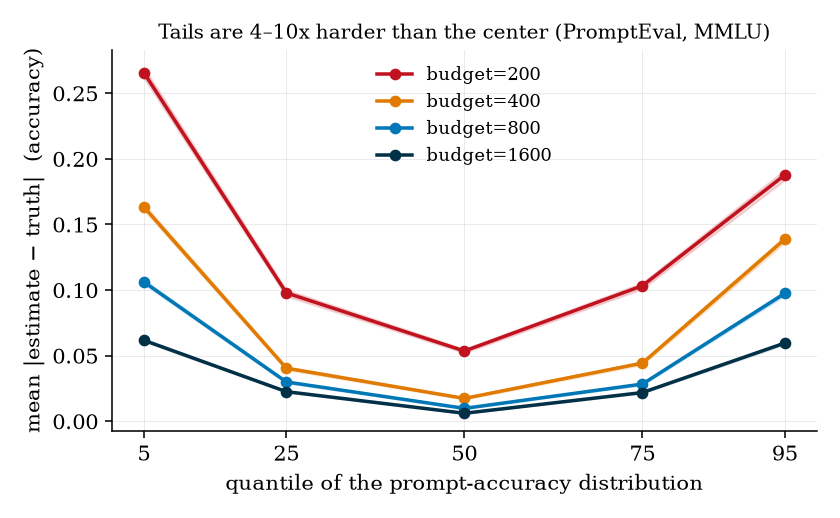
\includegraphics[width=0.62\textwidth]{fig1_center_vs_tail.png}
\caption{\pe{} error versus quantile on MMLU (mean $\pm$ bootstrap 95\% CI). The U-shape shows
the center--tail reliability gap at every budget.}
\label{fig:u}
\end{figure}

\section{Mechanism: directional over-dispersion}\label{sec:mech}
Is the tail error just symmetric noise (``extreme quantiles are harder''), or something a
practitioner would be actively misled by? We decompose it by \emph{sign}
(Fig.~\ref{fig:disp}). The bias is strongly directional: the $5$th-percentile estimate is too
\emph{low} (signed error $-0.265$, CI $[-0.270,-0.261]$ at $B{=}200$) and the $95$th too
\emph{high} ($+0.187$, CI $[+0.184,+0.191]$). Equivalently, the estimated distribution is
\emph{over-dispersed}: in $100\%$ of cells the estimated inter-quantile spread exceeds the
truth, with a median spread ratio of $8.4\times$ at $B{=}200$, still $3.1\times$ at $B{=}1600$.
This is counterintuitive: a regularized shrinkage estimator might be expected to
\emph{under}-state spread, but at practical budgets the sampling noise in the per-template
ability estimates $\hat\theta_p$ dominates and inflates the tails.

The consequence is decision-relevant. A practitioner reading \pe{} at $B{=}200$ would conclude
that their worst template is $\sim\!26$ accuracy points worse than it truly is, and that the
model is far more prompt-sensitive than it is. For best-\emph{prompt} selection, the template
\pe{} labels best is on average $3.5$ points below the true best (regret $0.035$), barely
improving to $0.028$ at $B{=}1600$.

That the over-dispersion is a finite-sample artifact is confirmed by its monotone decay toward
$1$ as budget grows (Fig.~\ref{fig:disp}, and the spread-ratio sequence
$8.4\!\to\!6.0\!\to\!4.4\!\to\!3.1$). This both explains the effect and suggests a correction.

\begin{figure}[h]\centering
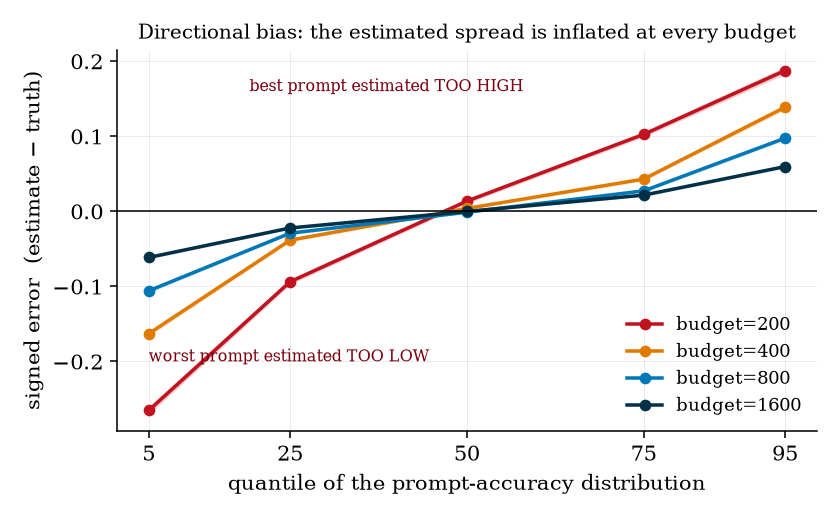
\includegraphics[width=0.62\textwidth]{fig2_overdispersion.png}
\caption{Signed error versus quantile. Low quantiles are underestimated and high quantiles
overestimated: the estimated prompt-sensitivity distribution is systematically over-dispersed.}
\label{fig:disp}
\end{figure}

\begin{figure}[h]\centering
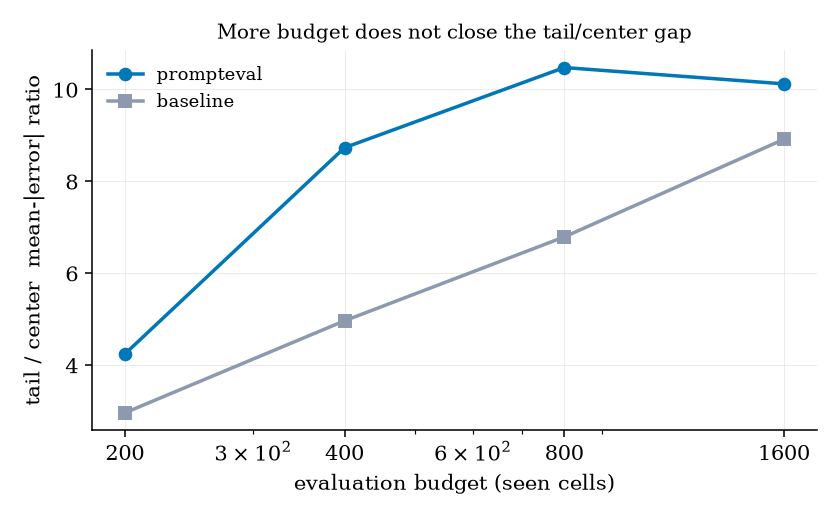
\includegraphics[width=0.55\textwidth]{fig3_tail_center_ratio.png}
\caption{The tail/center error ratio grows with budget: the reliability gap is not a
small-budget artifact.}
\label{fig:ratio}
\end{figure}

\section{A self-contained deconvolution correction}\label{sec:fix}
The diagnosis---noise-inflated spread---implies a fix. Let $s^\star$ be the factor by which the
\emph{true} per-template spread must be deflated so that, after the estimator's own inflation at
budget $B$, it matches the observed spread. We estimate $s^\star$ by a fixed-point parametric
bootstrap using only the budgeted data: (i) fit Eq.~\eqref{eq:rasch}; (ii) build a synthetic
truth by deflating the fitted $\hat\theta_p$ toward their mean by a factor $s$; (iii) simulate
$Y\!\sim\!\mathrm{Bernoulli}$ from it, re-run the same budgeted sampling and estimator, and
measure the inflation $\mathrm{infl}(s)=\mathrm{std}(\hat a^{\text{sim}})/\mathrm{std}(a^{\text{sim}})$;
(iv) update $s\leftarrow1/\mathrm{infl}(s)$ to a fixed point. We then shrink the real estimate,
$\hat a_p^{\text{corr}}=\bar a+s^\star(\hat a_p-\bar a)$, and recompute quantiles. The
correction uses \emph{no} additional labels and never sees the true quantiles.

On MMLU at $B{=}200$ the correction reduces tail ($q_5,q_{95}$) error from $0.189$ to $0.068$,
a $\mathbf{64\%}$ reduction, while also improving the center (Table~\ref{tab:fix}). Because it
shrinks toward the (well-estimated) mean, it cannot harm the median. It is deliberately
conservative---it recovers a $\sim\!2.8\times$ deflation rather than the full $\sim\!8\times$,
reflecting the fundamental difficulty of recovering a tiny true spread from ${\sim}2$ observed
items per template. This residual is itself the honest takeaway: at very small budgets the
tails should be corrected \emph{and} treated with caution.

\begin{table}[h]\centering\small
\caption{Deconvolution correction on MMLU at $B{=}200$ (mean $|$error$|$). It improves every
quantile and cuts tail error by $64\%$. [Full-grid numbers.]}
\label{tab:fix}
\begin{tabular}{lrrrrr}
\toprule
& $q_{5}$ & $q_{25}$ & $q_{50}$ & $q_{75}$ & $q_{95}$ \\
\midrule
\pe{} (orig)       & 0.234 & 0.074 & 0.035 & 0.072 & 0.143 \\
\pe{} + deconv     & 0.085 & 0.037 & 0.020 & 0.026 & 0.051 \\
reduction          & 64\% & 50\% & 43\% & 64\% & 65\% \\
\bottomrule
\end{tabular}
\end{table}

\section{Generalization}\label{sec:gen}
To test whether the effect is specific to MMLU's multiple-choice format, we repeat the
diagnosis on BBH (many free-form/reasoning tasks) and LMentry, using each benchmark's released
matrices ($187$ and $258$ templates respectively). Table~\ref{tab:gen} shows the pattern is
universal: at the headline budget the tail error is $2.4$--$4.2\times$ the center error on all
three benchmarks (paired Wilcoxon $p\le10^{-21}$), the estimate is over-dispersed in
$85$--$100\%$ of cells, and---as on MMLU---the tail/center ratio \emph{grows} with budget
rather than shrinking. The magnitude is largest on MMLU and smallest on LMentry, but the
direction (worst prompt too low and/or best prompt too high) never reverses.

\begin{table}[h]\centering\small
\caption{The center--tail gap and over-dispersion generalize across benchmarks (\pe{}).
``ratio'' is tail/center mean-$|$error$|$; ``o.d.\%'' is the fraction of cells whose estimated
spread exceeds the truth (cells with true spread $\ge0.02$).}
\label{tab:gen}
\begin{tabular}{lccccccc}
\toprule
& \multicolumn{3}{c}{$B{=}200$ (headline)} & & \multicolumn{2}{c}{$B{=}1600$} \\
\cmidrule(lr){2-4}\cmidrule(lr){6-7}
benchmark & $q_{50}$ err & tail err & ratio & o.d.\% & $q_{50}$ err & ratio \\
\midrule
MMLU (MCQ)        & 0.053 & 0.227 & $4.2\times$ & 100 & 0.006 & $10.1\times$ \\
BBH (free-form)   & 0.070 & 0.198 & $2.8\times$ & 93  & 0.015 & $6.0\times$ \\
LMentry           & 0.059 & 0.142 & $2.4\times$ & 85  & 0.022 & $3.4\times$ \\
\bottomrule
\end{tabular}
\end{table}

\section{Related work}
Prompt sensitivity of LLM benchmarks is well documented
\citep{sclar2024quantifying,mizrahi2024state}, motivating multi-prompt evaluation and \pe{}
\citep{polo2024prompteval}. A parallel psychometric line applies item-response theory to LLM
evaluation for efficiency and validity \citep{madaan2024quantifying}. Our work is a targeted
reproduction and stress-test in the spirit of ``sober-look'' evaluations: we confirm the
method's central-tendency claims and expose a specific, decision-relevant tail failure plus a
remedy. Concurrent work questions tail-focused metrics in a different setting (toxicity
reward-model extreme-value tails) \citep{tailfragile2026}; our over-dispersion mechanism and
deconvolution correction for multi-prompt performance quantiles are, to our knowledge,
unreported.

\section{Limitations}
Our study is a re-analysis of three released benchmarks with fixed template sets; the exact
magnitudes are specific to those matrices and to the Rasch estimator. The correction is a
variance (spread) correction and assumes the estimated \emph{mean} is approximately unbiased,
which holds empirically here. We analyze the released additive Rasch model; covariate-augmented
variants may behave differently, though they share the additive-in-logits structure.

\section{Conclusion}
Multi-prompt evaluation delivers on its central promise but not on its tails: the very
quantiles that make a distribution more informative than a point estimate are the least
reliable, systematically over-dispersed, and not fixed by more budget. We give a diagnosis, a
mechanism, and a label-free correction. The practical rule is simple: \emph{trust the center,
correct or distrust the edges.}

\paragraph{Reproducibility.} All code, the exact-match reproduction, and figure-generating
scripts run on a laptop from the authors' public data; see the repository.

\small
\bibliographystyle{plainnat}
\begin{thebibliography}{9}
\bibitem[Polo et al.(2024)]{polo2024prompteval} F.~Maia Polo et al.
\newblock Efficient multi-prompt evaluation of LLMs. \emph{NeurIPS}, 2024. arXiv:2405.17202.
\bibitem[Sclar et al.(2024)]{sclar2024quantifying} M.~Sclar et al.
\newblock Quantifying language models' sensitivity to spurious features in prompt design. \emph{ICLR}, 2024.
\bibitem[Mizrahi et al.(2024)]{mizrahi2024state} M.~Mizrahi et al.
\newblock State of what art? A call for multi-prompt LLM evaluation. \emph{TACL}, 2024.
\bibitem[Madaan et al.(2024)]{madaan2024quantifying} L.~Madaan et al.
\newblock Quantifying variance in evaluation benchmarks. 2024. arXiv:2406.10229.
\bibitem[Anonymous(2026a)]{rankintervals2026} Rank intervals for leaderboards: a hierarchical framework for model evaluation. 2026. arXiv:2606.08679.
\bibitem[Anonymous(2026b)]{tailfragile2026} Tail-shape estimation in LLM evaluation is fragile. 2026. arXiv:2606.16511.
\end{thebibliography}

\end{document}
